\documentclass{article}
\usepackage{tikz}
\usetikzlibrary{positioning, arrows.meta}

\begin{document}

\begin{tikzpicture}[node distance=1cm, auto]
    % Define nodes
    \node (image) [draw, rectangle] {Image};
    \node (patch) [right=of image, draw, rectangle, minimum width=2cm, minimum height=4cm] {Patch Embedding};
    \node (stage1) [right=of patch, draw, rectangle, minimum width=2cm, minimum height=2cm] {Stage 1};
    \node (cn1) [right=of stage1, draw, rectangle, minimum width=2cm, minimum height=2cm] {CN \\ $(7,7)$};
    \node (dl1) [right=of cn1, draw, rectangle, minimum width=2cm, minimum height=2cm] {downsampling Layer};
    \node (stage2) [right=of dl1, draw, rectangle, minimum width=2cm, minimum height=2cm] {Stage 2};
    \node (cn2) [right=of stage2, draw, rectangle, minimum width=2cm, minimum height=2cm] {CN \\ $(7,7)$};
    \node (dl2) [right=of cn2, draw, rectangle, minimum width=2cm, minimum height=2cm] {downsampling Layer};
    \node (stage3) [right=of dl2, draw, rectangle, minimum width=2cm, minimum height=2cm] {Stage 3};
    \node (cn3) [right=of stage3, draw, rectangle, minimum width=2cm, minimum height=2cm] {CN \\ $(7,7)$};
    \node (dl3) [right=of cn3, draw, rectangle, minimum width=2cm, minimum height=2cm] {downsampling Layer};
    \node (stage4) [right=of dl3, draw, rectangle, minimum width=2cm, minimum height=2cm] {Stage 4};
    \node (swin1) [right=of stage4, draw, rectangle, minimum width=2cm, minimum height=2cm] {Swin \\ $(5,40)$};
    \node (dl4) [right=of swin1, draw, rectangle, minimum width=2cm, minimum height=2cm] {downsampling Layer};
    \node (stage5) [right=of dl4, draw, rectangle, minimum width=2cm, minimum height=2cm] {Stage 5};
    \node (swin2) [right=of stage5, draw, rectangle, minimum width=2cm, minimum height=2cm] {Swin \\ $(5,20)$};
    \node (dl5) [right=of swin2, draw, rectangle, minimum width=2cm, minimum height=2cm] {downsampling Layer};
    \node (stage6) [right=of dl5, draw, rectangle, minimum width=2cm, minimum height=2cm] {Stage 6};
    \node (swin3) [right=of stage6, draw, rectangle, minimum width=2cm, minimum height=2cm] {Swin \\ $(10,10)$};

    % Draw connections
    \draw[->] (image) -- (patch);
    \draw[->] (patch) -- node[above] {$\times 3$} (stage1);
    \draw[->] (stage1) -- (cn1);
    \draw[->] (cn1) -- (dl1);
    \draw[->] (dl1) -- node[above] {$\times 6$} (stage2);
    \draw[->] (stage2) -- (cn2);
    \draw[->] (cn2) -- (dl2);
    \draw[->] (dl2) -- node[above] {$\times 6$} (stage3);
    \draw[->] (stage3) -- (cn3);
    \draw[->] (cn3) -- (dl3);
    \draw[->] (dl3) -- node[above] {$\times 2$} (stage4);
    \draw[->] (stage4) -- (swin1);
    \draw[->] (swin1) -- (dl4);
    \draw[->] (dl4) -- node[above] {$\times 2$} (stage5);
    \draw[->] (stage5) -- (swin2);
    \draw[->] (swin2) -- (dl5);
    \draw[->] (dl5) -- node[above] {$\times 2$} (stage6);
    \draw[->] (stage6) -- (swin3);

    % Add labels above each stage
    \node[above=0.5cm of stage1] {$\frac{H}{4}\cdot\frac{W}{4}\cdot C_{0}$};
    \node[above=0.5cm of stage2] {$\frac{H}{8}\cdot\frac{W}{4}\cdot C_{1}$};
    \node[above=0.5cm of stage3] {$\frac{H}{16}\cdot\frac{W}{4}\cdot C_{2}$};
    \node[above=0.5cm of stage4] {$\frac{H}{32}\cdot\frac{W}{8}\cdot C_{3}$};
    \node[above=0.5cm of stage5] {$\frac{H}{32}\cdot\frac{W}{16}\cdot C_{4}$};
    \node[above=0.5cm of stage6] {$\frac{H}{32}\cdot\frac{W}{32}\cdot C_{5}$};
    \node[above=0.5cm of swin3] {$\frac{H}{32}\cdot\frac{W}{32}\cdot C_{5}$};
\end{tikzpicture}

\end{document}